\chapter{CMR}

We have named the system \emph{CMR}, short for \emph{Concurrent Memory Reclamation}. The system is
implemented as a Rust library \code{cmr}. We have also implemented four data structures, a stack,
queue, list, and hasmap, in the \code{cmr-data-structures} library, which uses \code{cmr}
internally for memory reclamation.

This chapter is organized as follows:
Section~\ref{sec:cmr-overview} gives an overview of the system as a whole, and defines the problem
we want to solve.
Section~\ref{sec:cmr-primitives} defines the primitives of the system, how they interact, and
proves their correctness.
\todo{bla}

\section{Problem Definition}

We define an abstract model of the system, and prove its correctness.
The computational model we are working with is the RAM machine, and assume that
the reader is familiar with it\footnote{\todo{Have def.\ in background?}}.

We start by defining some central concepts.
Memory $M$ is the set of all addresses in the address space of the machine.
It is a disjoint set $M = A \cap F$ where $A$ is the set of allocated memory, and $F$ is the
remaining of the memory space.
A \emph{block} is a tuple $(addr, size)$ and represents the memory segment $[addr, addr + size)$.
We call memory that is in an allocated block \emph{valid memory}.

In Rust, most memory management is handled automatically by the compiler. CMR utilizes this by
distinguishing between \emph{Rust memory} and \emph{Shared memory}. Rust memory is all memory that
is managed by the compiler, for instance through smart pointers. Shared memory is the remaining
memory, which is managed by CMR\@. Note that there is a thin line in between the two types: types may
be handled by CMR, but they themselves may contain smart pointers which is then handled by Rust.
For instance, a node in a linked list implemented using CMR may contain data that contains a smart
pointer. When the node is freed, its destructor is ran, and the smart pointers cleanup is handled
just as if it was not in shared memory (see Figure~\ref{fig:rust-shared-mem}).

Since Rust manages Rust memory, we only need to do reachability queries in the shared memory
subset. For many applications, this is a much smaller space than the total memory. It is also
possible to have the data types that are referenced from shared memory but stored in Rust memory
(like the binary tree in Figure~\ref{fig:rust-shared-mem}) know whether they have pointers to
shared memory, so that we don't have to scan through the strucutre, as it may be arbitrary large.


\begin{figure}
  \centering
  \begin{tikzpicture}
  \node [lnode,node distance=1.5cm] (n1)               {};
  \node [lnode,node distance=1.5cm] (n2) [right of=n1] {};
  \node [lnode,node distance=1.5cm] (n3) [right of=n2] {};
  \node [lnode,node distance=1.5cm] (n4) [right of=n3] {};

  \draw[ptr] ($(n1.east) - (0.25,0)$) -- (n2);
  \draw[ptr] ($(n2.east) - (0.25,0)$) -- (n3);
  \draw[ptr] ($(n3.east) - (0.25,0)$) -- (n4);
  \draw[ptr] ($(n4.east) - (0.25,0)$) -- ($(n4.east) + (0.4,0)$);

  \node [draw,fill=white,node distance=1.5cm, inner sep=0.2cm] (d1) [below of=n1,xshift=-0.19cm] {};
  \node [draw,fill=white,node distance=2cm,circle] (d2) [below of=n2,xshift=-0.19cm] {};
  \node [draw,fill=white,node distance=1.5cm] (d3) [below of=n3,xshift=-0.19cm] {$\pi$};
  \node [draw,fill=white,node distance=1.5cm] (d4) [below of=n4,xshift=-0.19cm] {\code{"hello"}};


  \draw[ptr] ($(n1) + (-0.19, +0.05)$) -- (d1.north);
  \draw[ptr] ($(n2) + (-0.19, +0.05)$) -- (d2.north);
  \draw[ptr] ($(n3) + (-0.19, +0.05)$) -- (d3.north);
  \draw[ptr] ($(n4) + (-0.19, +0.05)$) -- (d4.north);

  \node[draw,fill=white,circle,node distance=0.5cm] (treel) [below of=d2,left of=d2] {};
  \node[draw,fill=white,circle,node distance=0.5cm] (treer) [below of=d2,right of=d2] {};
  \draw[-latex] (d2) -- (treel);
  \draw[-latex] (d2) -- (treer);

  \node [draw,fill=white,node distance=2cm] (back) [left of=n1] {\code{0xcafe}};
  \draw[ptr] (back) ($(d1) + (0.05,0)$) to [out=180,in=270] (back.south);

  \begin{scope}[on background layer]
    \node [draw,fill=lightred!40, fit={(back) (n4)},inner sep=0.5cm] (shared-mem) {};
    \node [draw,fill=rust!60, fit={(d1) (treel) (d4)},inner sep=0.3cm] (shared-mem) {};
  \end{scope}

  \node (shared-label) [above of=back] {Shared memory};
  \node (rust-label) [below of=d4,xshift=-0.3cm] {Owned memory};
\end{tikzpicture}

  \caption{Example of memory layout showing Rust memory (brown) and shared memory (red). Types in
  shared memory may contain pointers to Rust memory, and vice versa.\label{fig:rust-shared-mem}}
\end{figure}

We first define three memory hazards:

\begin{definition}[invalid-read]
  Memory that has never been allocated is read.
\end{definition}

\begin{definition}[use-after-free]
  Memory that was allocated and then freed is read.
\end{definition}

\begin{definition}[double-free]
  A block is freed twice without being allocated in between.
\end{definition}

We would like our system to guarantee that neither of the three happens.

\section{Overview\label{sec:cmr-overview}}

The high level idea of the system is for the consolidator to have easy access to all roots in every
thread. With this information, the problem of identifying garbage is equivalent to reachability
analysis in a graph in which the vertices are data types in the program and the edges are pointers.
 Having this, we can
identify the reachable segments $R \subseteq M$ and the garbage $G = M \setminus R$.

\begin{figure}[ht]
  \centering
  \begin{subfigure}{0.45\textwidth}
    \begin{lstlisting}
a = Node { value = 4, next = null }
b = Node { value = 8, next = a }
list = [a, b, 3]
    \end{lstlisting}
  \end{subfigure}
  \hfill
  \begin{subfigure}{0.45\textwidth}
    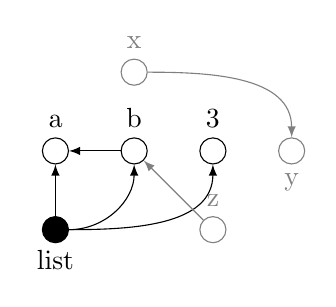
\begin{tikzpicture}[node distance=1cm]
  \node [draw,circle,label={a}]    (a)              {};

  \node [draw,circle,label={b}]    (b) [right of=a] {};
  \draw[-latex] (b.west) -- (a.east);

  \node [draw,circle,label={3}]    (3) [right of=b] {};

  \node [draw,circle,fill,label={[label distance=-0.8cm]:list}] (l) [below of=a] {};
  \draw[-latex] (l.north) -- (a.south);
  \draw[-latex] (l.east) to [out=0,in=270] (b.south);
  \draw[-latex] (l.east) to [out=0,in=270] (3.south);


  \node [draw,circle,color=gray,label={[color=gray]x}] (x) [above of=b] {};
  \node [draw,circle,color=gray,label={[color=gray,label distance=-0.8cm]y}] (y) [right of=3] {};
  \draw[-latex,color=gray] (x.east) to [out=0,in=90] (y.north);
  \node [draw,circle,color=gray,label={[color=gray]z}] (z) [below of=3] {};
  \draw[-latex,color=gray] (z) -- (b);
\end{tikzpicture}

  \end{subfigure}
  \caption{Code sample (left) with possible heap layout (right). If the black filled node is the
  only root, the black nodes are reachable, and the gray nodes are not. Note that one node (z)
  points to a reachable node, but is itself not reachable.}
\end{figure}

Performing the reachability analisys is not straight forwards, even when we have all roots in the
system. Consider a mark-and-sweep approach, where we follow pointers and keep track of memory
locations that we have seen before. Since we are running a concurrent system, pointers might be
updated while we scan, so that two pointer values might be swapped after looking at either of them,
making the other value invisible to the system, and causing memory to be registered as unreachable,
when it is not. See Figure~\ref{fig:pointer-swap} for an example.

\begin{figure}[ht]
  \centering
  \hfill
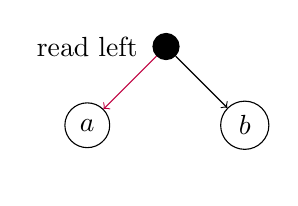
\begin{tikzpicture}
  \node [draw,fill,circle] (r) {};
  \node [draw,circle] (a) [left  of=r, below of=r] {$a$};
  \draw[->,color=purple] (r) -- (a);
  \node [draw,circle] (b) [right of=r, below of=r] {$b$};
  \draw[->] (r) -- (b);
  \draw[<->,color=white] (a) to [out=-45,in=-135] (b);

  \node () [left of=r] {read left};
\end{tikzpicture}
\hfill
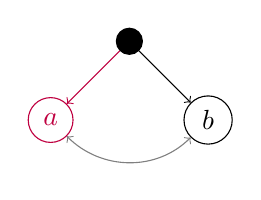
\begin{tikzpicture}
  \node [draw,fill,circle] (r) {};
  \node [draw,color=purple,circle] (a) [left  of=r, below of=r] {$a$};
  \draw[->,color=purple] (r) -- (a);
  \node [draw,circle] (b) [right of=r, below of=r] {$b$};
  \draw[->] (r) -- (b);
  \draw[<->,color=gray] (a) to [out=-45,in=-135] (b);
\end{tikzpicture}
\hfill
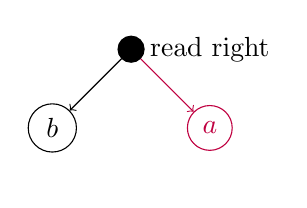
\begin{tikzpicture}
  \node [draw,fill,circle] (r) {};
  \node [draw,color=purple,circle] (a) [right  of=r, below of=r] {$a$};
  \draw[->,color=purple] (r) -- (a);
  \node [draw,circle] (b) [left of=r, below of=r] {$b$};
  \draw[->] (r) -- (b);
  \draw[<->,color=white] (b) to [out=-45,in=-135] (a);

  \node () [right of=r] {read right};
\end{tikzpicture}
\hfill

  \caption{Illustration of how mutation in the reachability graph can make a block $b$ appear as
  non-reachable. After we have looked at the roots left child, but before reading its right, the
  nodes child pointers are swapped. Since we cannot detect this (the two pointers could have been
  the same), we see $a$ twice and do not see $b$.\label{fig:pointer-swap}}
\end{figure}

In order to handle mutation problems, we obtain a snapshot of the entire processes memory by
freezing all threads, reading their roots, and forking the process. Thus, we have a snapshot of
the entire memory of the program, in which we also have all roots. Now the reachability analysis is
simpler, since there will be only one thread in the forked process, namely the garbage collecting
thread. Listing~\ref{lst:cmr} shows pseudocode for both the reclaiming thread and the other threads
for this procedure.

\begin{figure}[ht]
  \begin{subfigure}{0.45\textwidth}
    \begin{lstlisting}
CMR():
    freeze_threads()
    wait_for_writes()
    read_guards()
    fork()
    unfreeze()
    for addr in unreachables():
        free(addr)
    \end{lstlisting}
  \end{subfigure}
  \hfill
  \begin{subfigure}{0.45\textwidth}
    \begin{lstlisting}
on_freeze():
    write_roots()
    register_done()
    wait_for_unfreeze()
    \end{lstlisting}
  \end{subfigure}
  \caption{Pseudocode of CMR\@. The leftmost code is for the thread that runs the reclamation pass,
  and the rightmost code is other threads in the system.\label{lst:cmr}}
\end{figure}


\todo{define ``Rust memory'' and shared memory}

\section{Primitives of CMR\label{sec:cmr-primitives}}

The central data type to achieve this is \code{Guard}. A \code{Guard} is an object in which a
pointer to shared memory is stored. All pointers to shared memory are stored in a Guard. By
having access to all \code{Guard}s, CMR have access to all roots. \code{Guard}s are similar to
hazard pointers, except that no thread synchronization is performed when making new or updating
existing \code{Guard}s, which reduces the overhead significantly.

CMR has four types that are essential to understanding how we manage safe access to shared memory:
\emph{Guard}, \emph{Atomic}, \emph{NullablePtr}, and \emph{Ptr}. All types are generic over the
same type, which is omitted for brevity. We look at each type in turn.

\begin{definition}[Guard]
  A \emph{Guard} is an object that contains a \emph{root}. The Guard is non-movable in memory.
  All roots are stored in Guards.
\end{definition}

\begin{definition}[Atomic]
  An \emph{Atomic} is a pointer variable that provides safe concurrent access.
\end{definition}

\begin{definition}[NullablePtr]
  \emph{NullablePtr} is an immutable pointer that may be $\bot$. It is obtained through a Guard.
  When a NullablePtr $p$ is obtained from a Guard $g$, $g$ is immutable thoughout the lifetime of
  $p$.
\end{definition}

\begin{definition}[Ptr]
  \emph{Ptr} is an immutable pointer that may \emph{not} be $\bot$. Its semantics are similar to
  that of NullablePtr, but the two are distinct types for simplification. All accesses to shared
  memory is through a Ptr.
\end{definition}


Having defined the types, we define the operations on the types:

\begin{definition}[Common operations]
\begin{equation}\label{eq:make-guard}
  \text{make-guard\:::\:} () \to Guard
\end{equation}
\emph{make-guard} constructs a new Guard variable containing $\bot$.

\begin{equation}\label{eq:load-atomic}
  \text{load-atomic\:::\:} (Guard, Atomic) \to NullablePtr
\end{equation}
\emph{load-atomic} reads the atomic vairable, protects it with the Guard, and return a NullablePtr
to the value read.
\end{definition}

\begin{definition}\label{def:atomic}
  $\text{atomic\:::\:} (() \to T) \to T$ is a higher order function that runs a function without
  a reclamation pass happening during the functions execution.
\end{definition}




With these types and operations we are able to prove important properties of the system.

\begin{theorem}[Guard is valid]\label{thm:guard-valid}
  If a Guard is not $\bot$, it points to valid memory.
\end{theorem}
\begin{proof}
  \note{lol}
  Assume the Guard $g$ $\neq \bot$.
  The Guard has loaded its value from an Atomic $a$ using $atomic-load$.
We first show that $a$ is itself in valid memory. By induction:
\emph{Base case:} the Atomic resides in Rust memory, and is thus valid. \emph{Inductive case:} the
Atomic resides in shared memory, and thus accessed through a Ptr $p$.  This Ptr is protected by a
Guard $g\sb{2} \neq g$, since $g\sb{2}$ is immutable throughout the lifetime of $p$, and $g$ is
being changed. $g\sb{2}$ is valid by induction, so the pointer value in $a$ is reachable.

Using Definition~\ref{def:atomic}, we make sure that the read of $a$ and the store in $g$ happens
without a reclamation pass in between. Thus all valid pointers before the read is still valid after
the store.  After the store operation in $g$ has completed, $g$ protects $v$. Thus $v$ is valid.
\end{proof}

\begin{lemma}[Ptr is valid]\label{lm:ptr-valid}
  The Ptr points to valid memory.
\end{lemma}
\begin{proof}
The  Ptr $p$ is read from a Guard $g$ and $g$ is immutable throughout the lifetime of $p$ so they
have the same value. $p \neq \bot$, so this follows by Theorem~\ref{thm:guard-valid}.
\end{proof}




\section{Implementation}

The key idea of the implementation is to use an operation known as \emph{forking} to obtain a
snapshot of the entire memory space of the process. Having this we can identify the roots, and run
reachability analysis, knowing that nothing will change while we are looking.

Consolidation starts by sending all running threads a \emph{signal}, causing them to jump to a
\emph{signal handler}. The signal handler registers that the thread has been signaled, such that the
garbage collection pass is detectable. Then the thread writes out the address of a thread local
list of allocated addresses, such that the consolidator can collect all addresses that has been
allocated since the last consolidation. At last, the threads wait for the consolidator to say that
they may return to their execution. \note{why is this required?}

\note{Add implementation details here}

  \code{WAS\_SIGNALED} is a thread local flag that is
  set to \code{true} in the signal handler. Note that this function does not support being called
  recursively.
\begin{figure}[ht]
  \begin{lstlisting}[numbers=left,numberstyle=\color{gray}\ttfamily{}A]
fn atomic(f: F):
  loop:
    WAS_SIGNALED = false
    let ret = f()
    if not WAS_SIGNALED: return ret
\end{lstlisting}
\caption{Pseudocode of $atomic$}
\end{figure}

\begin{theorem}
  If \code{f} does not itself call \code{atomic} then \code{atomic} satisfy
  Definition~\ref{def:atomic}.
\end{theorem}
\begin{proof}
  \code{WAS\_SIGNALED} is set to \code{false} in \code{A3}, so if it is observed to be
  \code{true} in \code{A5} the signal handler must have been executed. Since only the consolidator
  signals any thread, it means that there was a consolidator in this time interval. We are only
  returning from the function if \code{WAS\_SIGNALED = false}, so if we return \code{f} was
  successfully called without overlapping with a pass.
\end{proof}
Note that it is possible that the consolidator was initiated before entering the \code{atomic}
function, but that they only got execution time after \code{A3}.
\begin{lemma}
  If the consolidator is lock-free, then \code{atomic} is lock-free.
\end{lemma}
\begin{proof}
  If we loop, there is a consolidator. Since the consolidate process has a finite number of steps
  and is lock-free, it will either make progress, or some other thread is making progress. In
  either case, the system makes progress.
  \note{this is a terrible proof}
\end{proof}

It is important that the function given to \code{atomic} can be called multiple times without
breaking. The most useful case for \code{atomic} is a \code{load/store} store pair, so this is
usually the case.

